% answers.tex —— 2006 年·四川卷·文科 · 参考答案与详细解析片段
% 由 tools/generate_projects.py 依来源总账自 2006/2006_数学真题_四川文_试题.md + 2006/2006_数学真题_四川文_解析正文.md + 2006/2006_数学真题_四川文_答案要点.md 生成，勿手改（改源 MD 后重跑）


\begin{gktip}
以下解答依据固定 PDF 可见题面推导，不是卷内答案或官方解析。固定副本的发布者、版次、来源链及官方身份未核。
\end{gktip}

\begin{answer}
\gksolhead{1}{}

\textbf{题目}：

已知集合 $A=\{x\mid x^2-5x+6\leqslant0\}$，集合 $B=\{x\mid |2x-1|>3\}$，则集合 $A\cap B=$\mbox{（　　）}。

（A）$\{x\mid 2\leqslant x\leqslant3\}$　　（B）$\{x\mid 2\leqslant x<3\}$

（C）$\{x\mid 2<x\leqslant3\}$　　（D）$\{x\mid -1<x<3\}$

\Needspace{4\baselineskip}
\textbf{解析}

$A=[2,3]$，而$|2x-1|>3$等价于$x<-1$或$x>2$，故$A\cap B=(2,3]$，选C。

\gkanswer{答案：C}

\end{answer}
\begin{answer}
\gksolhead{2}{}

\textbf{题目}：

函数 $f(x)=\ln(x-1)\ (x>1)$ 的反函数是\mbox{（　　）}。

（A）$f^{-1}(x)=e^x+1\ (x\in\mathbb R)$　　（B）$f^{-1}(x)=10^x+1\ (x\in\mathbb R)$

（C）$f^{-1}(x)=10^x+1\ (x>1)$　　（D）$f^{-1}(x)=e^x+1\ (x>1)$

\Needspace{4\baselineskip}
\textbf{解析}

令$y=\ln(x-1)$，交换$x,y$并解出原自变量，得反函数$y=e^x+1$，定义域为$\mathbb R$，选A。

\gkanswer{答案：A}

\end{answer}
\begin{answer}
\gksolhead{3}{}

\textbf{题目}：

曲线 $y=4x-x^3$ 在点 $(-1,-3)$ 处的切线方程是\mbox{（　　）}。

（A）$y=7x+4$　　（B）$y=7x+2$　　（C）$y=x-4$　　（D）$y=x-2$

\Needspace{4\baselineskip}
\textbf{解析}

$y'=4-3x^2$，在$x=-1$处斜率为1。过$(-1,-3)$的切线为$y+3=x+1$，即$y=x-2$，选D。

\gkanswer{答案：D}

\end{answer}
\begin{answer}
\gksolhead{4}{}

\textbf{题目}：

如图，已知正六边形 $P_1P_2P_3P_4P_5P_6$，下列向量的数量积中最大的是\mbox{（　　）}。
\nopagebreak[4]
\begin{center}% Q4: regular hexagon from the fixed candidate PDF, printed page 334.
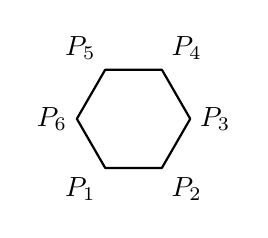
\begin{tikzpicture}[line cap=round,line join=round,x=0.72cm,y=0.72cm]
  \coordinate (P1) at (0,0);
  \coordinate (P2) at (1,0);
  \coordinate (P3) at (1.5,0.866);
  \coordinate (P4) at (1,1.732);
  \coordinate (P5) at (0,1.732);
  \coordinate (P6) at (-0.5,0.866);
  \draw[thick] (P1)--(P2)--(P3)--(P4)--(P5)--(P6)--cycle;
  \node[below left] at (P1) {$P_1$};
  \node[below right] at (P2) {$P_2$};
  \node[right] at (P3) {$P_3$};
  \node[above right] at (P4) {$P_4$};
  \node[above left] at (P5) {$P_5$};
  \node[left] at (P6) {$P_6$};
\end{tikzpicture}
\end{center}
\nopagebreak[4]
（A）$\overrightarrow{P_1P_2}\cdot\overrightarrow{P_1P_3}$　　（B）$\overrightarrow{P_1P_2}\cdot\overrightarrow{P_1P_4}$

（C）$\overrightarrow{P_1P_2}\cdot\overrightarrow{P_1P_5}$　　（D）$\overrightarrow{P_1P_2}\cdot\overrightarrow{P_1P_6}$

\Needspace{4\baselineskip}
\textbf{解析}

设正六边形边长为$s$。四个数量积依次为$\frac32s^2,s^2,0,-\frac12s^2$，最大值对应$\overrightarrow{P_1P_3}$，选A。

\gkanswer{答案：A}

\end{answer}
\begin{answer}
\gksolhead{5}{}

\textbf{题目}：

甲校有3600名学生，乙校有5400名学生，丙校有1800名学生，为统计三校学生某方面的情况，计划采用分层抽样法，抽取一个容量为90人的样本，应在这三校分别抽取学生\mbox{（　　）}。

（A）30人，30人，30人　　（B）30人，45人，15人

（C）20人，30人，10人　　（D）30人，50人，10人

\Needspace{4\baselineskip}
\textbf{解析}

总人数为10800，抽样比例为$90/10800=1/120$，故三校分别抽取30、45、15人，选B。

\gkanswer{答案：B}

\end{answer}
\begin{answer}
\gksolhead{6}{}

\textbf{题目}：

下列函数中，图象的一部分如图所示的是\mbox{（　　）}。
\nopagebreak[4]
\begin{center}% Q6: schematic cosine graph with the source's labelled intercept and maximum.
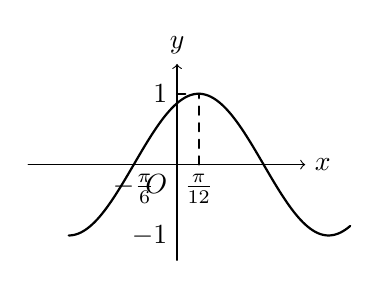
\begin{tikzpicture}[line cap=round,line join=round,x=1.05cm,y=0.9cm]
  \draw[->] (-1.8,0)--(1.55,0) node[right] {$x$};
  \draw[->] (0,-1.35)--(0,1.42) node[above] {$y$};
  \draw[thick,dashed] ({pi/12},0)--({pi/12},1);
  \draw[thick,dashed] (0,1)--({pi/12},1);
  \draw[thick,domain=-75:120,samples=120,variable=\t]
    plot ({\t*pi/180},{cos(2*\t-30)});
  \node[below left] at (0,0) {$O$};
  \node[left] at (0,1) {$1$};
  \node[left] at (0,-1) {$-1$};
  \node[below] at ({-pi/6},0) {$-\frac{\pi}{6}$};
  \node[below] at ({pi/12},0) {$\frac{\pi}{12}$};
\end{tikzpicture}
\end{center}
\nopagebreak[4]
（A）$y=\sin\left(x+\dfrac\pi6\right)$　　（B）$y=\sin\left(2x-\dfrac\pi6\right)$

（C）$y=\cos\left(4x-\dfrac\pi3\right)$　　（D）$y=\cos\left(2x-\dfrac\pi6\right)$

\Needspace{4\baselineskip}
\textbf{解析}

图象在$x=\pi/12$处取最大值1，且$x=-\pi/6$为零点，符合$y=\cos(2x-\pi/6)$，选D。

\gkanswer{答案：D}

\end{answer}
\begin{answer}
\gksolhead{7}{}

\textbf{题目}：

已知二面角 $\alpha-l-\beta$ 的大小为 $60^\circ$，$m,n$ 为异面直线，且 $m\perp\alpha$，$n\perp\beta$，则 $m,n$ 所成的角为\mbox{（　　）}。

（A）$30^\circ$　　（B）$60^\circ$　　（C）$90^\circ$　　（D）$120^\circ$

\Needspace{4\baselineskip}
\textbf{解析}

$m,n$分别垂直于两平面，其方向与两平面的法线平行；二面角为$60^\circ$，故两直线所成角为$60^\circ$，选B。

\gkanswer{答案：B}

\end{answer}
\begin{answer}
\gksolhead{8}{}

\textbf{题目}：

已知两定点 $A(-2,0)$、$B(1,0)$，如果动点 $P$ 满足 $|PA|=2|PB|$，则点 $P$ 的轨迹所围图形的面积等于\mbox{（　　）}。

（A）$9\pi$　　（B）$8\pi$　　（C）$4\pi$　　（D）$\pi$

\Needspace{4\baselineskip}
\textbf{解析}

由$PA=2PB$得$(x+2)^2+y^2=4((x-1)^2+y^2)$，化为圆心$(2,0)$、半径2的圆，面积为$4\pi$，选C。

\gkanswer{答案：C}

\end{answer}
\begin{answer}
\gksolhead{9}{}

\textbf{题目}：

如图，正四棱锥 $P-ABCD$ 底面的四个顶点 $A\text{、}B\text{、}C\text{、}D$ 在球 $O$ 的同一个大圆上，点 $P$ 在球面上，如果 $V_{P-ABCD}=\dfrac{16}{3}$，则球 $O$ 的表面积是\mbox{（　　）}。
\nopagebreak[4]
\begin{center}% Q9: sphere containing a regular square pyramid whose base lies in a great circle.
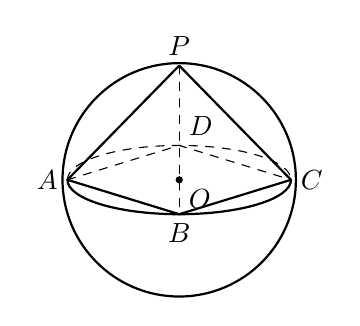
\begin{tikzpicture}[line cap=round,line join=round,x=0.78cm,y=0.78cm]
  \coordinate (O) at (0,0);
  \coordinate (P) at (0,1.86);
  \coordinate (A) at (-1.82,0);
  \coordinate (B) at (0,-0.56);
  \coordinate (C) at (1.82,0);
  \coordinate (D) at (0,0.56);
  \draw[thick] (O) circle (1.9);
  \draw[dashed] (A) arc[start angle=180,end angle=0,x radius=1.82,y radius=0.56];
  \draw[thick] (A) arc[start angle=180,end angle=360,x radius=1.82,y radius=0.56];
  \draw[thick] (A)--(B)--(C);
  \draw[dashed] (A)--(D)--(C);
  \draw[thick] (P)--(A) (P)--(C);
  \draw[dashed] (P)--(B) (P)--(D);
  \fill (O) circle (1.3pt);
  \node[above] at (P) {$P$};
  \node[left] at (A) {$A$};
  \node[below] at (B) {$B$};
  \node[right] at (C) {$C$};
  \node[above right] at (D) {$D$};
  \node[below right] at (O) {$O$};
\end{tikzpicture}
\end{center}
\nopagebreak[4]
（A）$4\pi$　　（B）$8\pi$　　（C）$12\pi$　　（D）$16\pi$

\Needspace{4\baselineskip}
\textbf{解析}

设球半径为$R$。底面正方形所在大圆过球心，正方形面积为$2R^2$，锥高为$R$。由$\frac13\cdot2R^2\cdot R=\frac{16}{3}$得$R=2$，球面面积为$16\pi$，选D。

\gkanswer{答案：D}

\end{answer}
\begin{answer}
\gksolhead{10}{}

\textbf{题目}：

直线 $y=x-3$ 与抛物线 $y^2=4x$ 交于 $A\text{、}B$ 两点，过 $A\text{、}B$ 两点向抛物线的准线作垂线，垂足分别为 $P\text{、}Q$，则梯形 $APQB$ 的面积为\mbox{（　　）}。

（A）36　　（B）48　　（C）56　　（D）64

\Needspace{4\baselineskip}
\textbf{解析}

联立$y=x-3$与$y^2=4x$得交点为$(1,-2),(9,6)$。抛物线准线为$x=-1$，两腰长分别为2和10，两平行底边间距为8，梯形面积为$\frac{2+10}{2}\cdot8=48$，选B。

\gkanswer{答案：B}

\end{answer}
\begin{answer}
\gksolhead{11}{}

\textbf{题目}：

设 $a\text{、}b\text{、}c$ 分别是 $\triangle ABC$ 的三个内角 $A\text{、}B\text{、}C$ 所对的边，则 $a^2=b(b+c)$ 是 $A=2B$ 的\mbox{（　　）}。

（A）充要条件　　（B）充分而不必要条件　　（C）必要而不充分条件　　（D）既不充分也不必要条件

\Needspace{4\baselineskip}
\textbf{解析}

由余弦定理，$a^2=b(b+c)$等价于$c/b=1+2\cos A$。由正弦定理及$C=\pi-A-B$，$c/b=\sin(A+B)/\sin B=\cos A+\sin A\cot B$，所以$\sin A\cot B=1+\cos A$，即$\cot B=\cot(A/2)$。其中$B,A/2\in(0,\pi/2)$，故$B=A/2$，即$A=2B$；反向代入亦成立，选A。

\gkanswer{答案：A}

\end{answer}
\begin{answer}
\gksolhead{12}{}

\textbf{题目}：

从0到9这10个数字中任取3个数字组成一个没有重复数字的三位数，这个数不能被3整除的概率为\mbox{（　　）}。

（A）$\dfrac{41}{60}$　　（B）$\dfrac{38}{54}$　　（C）$\dfrac{35}{54}$　　（D）$\dfrac{19}{54}$

\Needspace{4\baselineskip}
\textbf{解析}

全部无重复三位数共$9\cdot9\cdot8=648$个。按数字对3取余分类，三位数能被3整除的有228个（余数为$000,111,222$的同类组有30个，余数为$012$的组合有198个）。故不能被3整除的有420个，概率为$420/648=35/54$，选C。

\gkanswer{答案：C}

\end{answer}
\begin{answer}
\gksolhead{13}{}

\textbf{题目}：

$(1-2x)^{10}$ 展开式中的 $x^3$ 的系数为\gkblank{}。（用数字作答）

\Needspace{4\baselineskip}
\textbf{解析}

$x^3$项系数为$\binom{10}{3}(-2)^3=-960$。

\gkanswer{答案：$-960$}

\end{answer}
\begin{answer}
\gksolhead{14}{}

\textbf{题目}：

\Needspace{5\baselineskip}
设 $x,y$ 满足约束条件
\nopagebreak[4]
\[
\begin{cases}
x\geqslant1,\\
y\geqslant\dfrac12x,\\
2x+y\leqslant10,
\end{cases}
\]
则 $z=2x-y$ 的最小值为\gkblank{}。

\Needspace{4\baselineskip}
\textbf{解析}

可行域顶点为$(1,\frac12),(1,8),(4,2)$，目标函数$z=2x-y$对应值为$\frac32,-6,6$，最小值为$-6$。

\gkanswer{答案：$-6$}

\end{answer}
\begin{answer}
\gksolhead{15}{}

\textbf{题目}：

如图，把椭圆 $\dfrac{x^2}{25}+\dfrac{y^2}{16}=1$ 的长轴 $AB$ 分成8等分，过每个分点作 $x$ 轴的垂线交椭圆的上半部分于 $P_1\text{、}P_2\text{、}\ldots\text{、}P_7$ 七个点，$F$ 是椭圆的一个焦点，则 $|P_1F|+|P_2F|+\cdots+|P_7F|=$\gkblank{}。
\nopagebreak[4]
\begin{center}% Q15: ellipse, eight equal major-axis intervals, seven upper-arc points, and a focus.
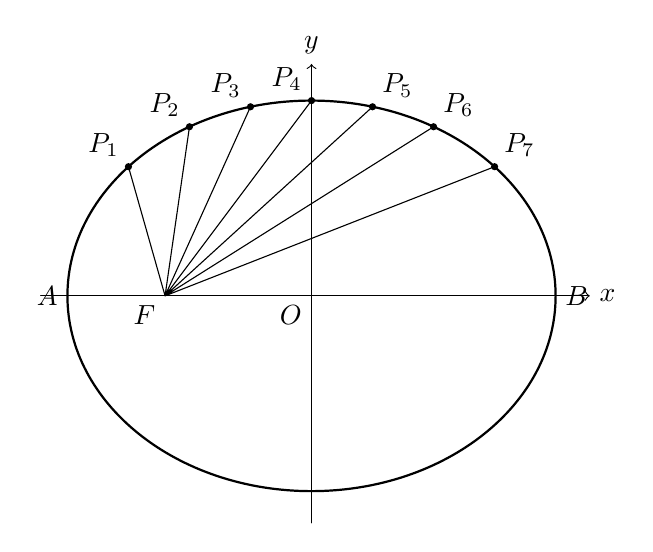
\begin{tikzpicture}[line cap=round,line join=round,x=0.62cm,y=0.62cm]
  \coordinate (P1) at (-3.75,2.646);
  \coordinate (P2) at (-2.50,3.464);
  \coordinate (P3) at (-1.25,3.873);
  \coordinate (P4) at (0,4);
  \coordinate (P5) at (1.25,3.873);
  \coordinate (P6) at (2.50,3.464);
  \coordinate (P7) at (3.75,2.646);
  \coordinate (F) at (-3,0);
  \draw[->] (-5.55,0)--(5.7,0) node[right] {$x$};
  \draw[->] (0,-4.65)--(0,4.75) node[above] {$y$};
  \draw[thick] (0,0) ellipse (5 and 4);
  \draw[thin] (F)--(P1) (F)--(P2) (F)--(P3) (F)--(P4)
              (F)--(P5) (F)--(P6) (F)--(P7);
  \foreach \i in {1,...,7} \fill (P\i) circle (1.3pt);
  \node[left] at (-5,0) {$A$};
  \node[right] at (5,0) {$B$};
  \node[below left] at (F) {$F$};
  \node[below left] at (0,0) {$O$};
  \node[above left] at (P1) {$P_1$};
  \node[above left] at (P2) {$P_2$};
  \node[above left] at (P3) {$P_3$};
  \node[above left] at (P4) {$P_4$};
  \node[above right] at (P5) {$P_5$};
  \node[above right] at (P6) {$P_6$};
  \node[above right] at (P7) {$P_7$};
\end{tikzpicture}
\end{center}
\nopagebreak[4]
\Needspace{4\baselineskip}
\textbf{解析}

椭圆半长轴$a=5$、半焦距$c=3$。对焦点$F=(-3,0)$，椭圆上横坐标为$x$的点到$F$距离为$5+\frac35x$；对另一焦点则为$5-\frac35x$。七个分点横坐标关于0对称，和为0，故距离和为$7\cdot5=35$。

\gkanswer{答案：$35$}

\end{answer}
\begin{answer}
\gksolhead{16}{}

\textbf{题目}：

$m,n$ 是空间两条不同直线，$\alpha,\beta$ 是两个不同平面，下面有四个命题：

① $m\perp\alpha,\ n\parallel\beta,\ \alpha\parallel\beta\Rightarrow m\perp n$；

② $m\perp n,\ \alpha\parallel\beta,\ m\perp\alpha\Rightarrow n\parallel\beta$；

③ $m\perp n,\ \alpha\parallel\beta,\ m\parallel\alpha\Rightarrow n\perp\beta$；

④ $m\perp\alpha,\ m\parallel n,\ \alpha\parallel\beta\Rightarrow n\perp\beta$。

其中真命题的编号是\gkblank{}。（写出所有真命题的编号）

\Needspace{4\baselineskip}
\textbf{解析}

①由$m\perp\alpha$且$\alpha\parallel\beta$，知$m$垂直于$\beta$内任一直线方向，故$m\perp n$。②由$m\perp\alpha$且$n\perp m$，得$n\parallel\alpha$，进而$n\parallel\beta$。③不成立，例如$\alpha,\beta$取水平平行平面，$m$取水平方向而$n$取与$m$垂直的另一水平方向。④由$m\perp\alpha$、$n\parallel m$及$\alpha\parallel\beta$得$n\perp\beta$。故真命题为①②④。

\gkanswer{答案：①②④}

\end{answer}
\begin{answer}
\gksolhead{17}{}

\textbf{题目}：

数列 $\{a_n\}$ 的前 $n$ 项和记为 $S_n$，$a_1=1$，$a_{n+1}=2S_n+1\ (n\geqslant1)$。

（1） 求 $\{a_n\}$ 的通项公式；

（2） 等差数列 $\{b_n\}$ 的各项为正，其前 $n$ 项和为 $T_n$，且 $T_3=15$，又 $a_1+b_1,a_2+b_2,a_3+b_3$ 成等比数列，求 $T_n$。

\Needspace{4\baselineskip}
\textbf{解析}

\textbf{(1)} $a_2=2a_1+1=3$。由$a_{n+1}=2S_n+1$与$a_n=2S_{n-1}+1$相减得$a_{n+1}-a_n=2a_n$，所以$a_{n+1}=3a_n$，从而$a_n=3^{n-1}$。

\textbf{(2)} 设$b_n$首项为$u$、公差为$d$。$T_3=15$给出$u+d=5$，于是$a_1+b_1=1+u$、$a_2+b_2=8$、$a_3+b_3=19-u$。成等比数列要求$(1+u)(19-u)=64$，得$u=3$或15。各项为正排除$u=15$，故$b_1=3,d=2$，$T_n=\frac n2(2b_1+(n-1)d)=n(n+2)$。

\gkanswer{答案（1）：$a_n=3^{n-1}$}

\gkanswer{答案（2）：$T_n=n(n+2)$}

\end{answer}
\begin{answer}
\gksolhead{18}{}

\textbf{题目}：

已知 $A\text{、}B\text{、}C$ 是 $\triangle ABC$ 三内角，向量 $\vec m=(-1,\sqrt3)$，$\vec n=(\cos A,\sin A)$，且 $\vec m\cdot\vec n=1$。

（1） 求角 $A$；

（2） 若 $\dfrac{1+\sin2B}{\cos^2B-\sin^2B}=-3$，求 $\tan C$。

\Needspace{4\baselineskip}
\textbf{解析}

\textbf{(1)} 点积条件为$-\cos A+\sqrt3\sin A=1$，即$2\sin(A-30^\circ)=1$。结合$0<A<180^\circ$，得$A=60^\circ$。

\textbf{(2)} 令$t=\tan B$，题设等式化为$(t+1)^2/(1-t^2)=-3$，得$t=2$或$-1$。因$B+C=120^\circ$，$B=-45^\circ$模$180^\circ$不符合内角范围，故$\tan B=2$。于是$\tan C=\tan(120^\circ-B)=\frac{8+5\sqrt3}{11}$。

\gkanswer{答案（1）：$A=60^\circ$}

\gkanswer{答案（2）：$\tan C=\dfrac{8+5\sqrt3}{11}$}

\end{answer}
\begin{answer}
\gksolhead{19}{}

\textbf{题目}：

某课程考核分理论和实验两部分进行，每部分考核成绩只记“合格”与“不合格”，两部分考核都“合格”则该课程考核“合格”。甲、乙、丙三人在理论考核中合格的概率分别为0.9、0.8、0.7；在实验考核中合格的概率分别为0.8、0.7、0.9。所有考核是否合格互相之间没有影响。

（1） 求甲、乙、丙三人在理论考核中至少有两人合格的概率；

（2） 求这三人该课程考核都合格的概率。（结果保留三位小数）

\Needspace{4\baselineskip}
\textbf{解析}

\textbf{(1)} 理论考核恰有两人合格的概率为$0.216+0.126+0.056=0.398$，三人均合格的概率为$0.9\cdot0.8\cdot0.7=0.504$，合计$0.902$。

\textbf{(2)} 三人课程考核合格概率分别为$0.9\cdot0.8$、$0.8\cdot0.7$、$0.7\cdot0.9$。相互独立，三人均合格概率为$0.72\cdot0.56\cdot0.63=0.254016$，保留三位小数为$0.254$。

\gkanswer{答案（1）：$0.902$}

\gkanswer{答案（2）：$0.254$}

\end{answer}
\begin{answer}
\gksolhead{20}{}

\textbf{题目}：

如图，在长方体 $ABCD-A_1B_1C_1D_1$ 中，$E\text{、}P$ 分别是 $BC\text{、}A_1D_1$ 的中点，$M\text{、}N$ 分别是 $AE\text{、}CD_1$ 的中点，$AD=AA_1=a$，$AB=2a$。

（1） 求证：$MN\parallel$ 平面 $ADD_1A_1$；

（2） 求二面角 $P-AE-D$ 的大小。
\nopagebreak[4]
\begin{center}% Q20: cuboid with the marked midpoints and required segments.
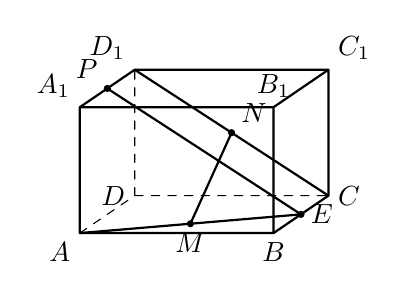
\begin{tikzpicture}[line cap=round,line join=round,x=0.82cm,y=0.82cm]
  \coordinate (A) at (0,0);
  \coordinate (B) at (3,0);
  \coordinate (C) at (3.85,0.58);
  \coordinate (D) at (0.85,0.58);
  \coordinate (Aone) at (0,1.95);
  \coordinate (Bone) at (3,1.95);
  \coordinate (Cone) at (3.85,2.53);
  \coordinate (Done) at (0.85,2.53);
  \coordinate (P) at (0.425,2.24);
  \coordinate (E) at (3.425,0.29);
  \coordinate (M) at (1.7125,0.145);
  \coordinate (N) at (2.35,1.555);

  % Rear edges are dashed; the front and right faces remain visible.
  \draw[dashed] (A)--(D) (D)--(C) (D)--(Done);
  \draw[thick] (A)--(B)--(C) (B)--(Bone)--(Cone)--(C)
               (A)--(Aone) (Aone)--(Bone) (Aone)--(Done)--(Cone) (A)--(B);
  \draw[thick] (A)--(E) (C)--(Done) (M)--(N) (P)--(E);
  \fill (P) circle (1.3pt) (E) circle (1.3pt) (M) circle (1.3pt) (N) circle (1.3pt);
  \node[below left] at (A) {$A$};
  \node[below] at (B) {$B$};
  \node[right] at (C) {$C$};
  \node[left] at (D) {$D$};
  \node[above left] at (Aone) {$A_1$};
  \node[above] at (Bone) {$B_1$};
  \node[above right] at (Cone) {$C_1$};
  \node[above left] at (Done) {$D_1$};
  \node[above left] at (P) {$P$};
  \node[right] at (E) {$E$};
  \node[below] at (M) {$M$};
  \node[above right] at (N) {$N$};
\end{tikzpicture}
\end{center}
\nopagebreak[4]
\Needspace{4\baselineskip}
\textbf{解析}

\textbf{(1)} 取$A=(0,0,0),B=(2a,0,0),D=(0,a,0),A_1=(0,0,a)$。则$E=(2a,a/2,0)$、$P=(0,a/2,a)$、$M=(a,a/4,0)$、$N=(a,a,a/2)$。故$\overrightarrow{MN}=(0,3a/4,a/2)$平行于平面$ADD_1A_1$，结论成立。

\textbf{(2)} 平面$DAE$的法向量可取$(0,0,1)$，平面$PAE$的法向量可取$(1,-4,2)$。两法向量夹角余弦为$2/\sqrt{21}$，故所求二面角为$\arccos(2/\sqrt{21})$。

\gkanswer{答案（1）：见解析版}

\gkanswer{答案（2）：$\arccos\dfrac2{\sqrt{21}}$}

\end{answer}
\begin{answer}
\gksolhead{21}{}

\textbf{题目}：

已知函数 $f(x)=x^3+3ax-1$，$g(x)=f'(x)-ax-5$，其中 $f'(x)$ 是 $f(x)$ 的导函数。

（1） 对满足 $-1\leqslant a\leqslant1$ 的一切 $a$ 值，都有 $g(x)<0$，求实数 $x$ 的取值范围；

（2） 设 $a=-m^2$，当实数 $m$ 在什么范围内变化时，函数 $y=f(x)$ 的图象与直线 $y=3$ 只有一个公共点。

\Needspace{4\baselineskip}
\textbf{解析}

\textbf{(1)} $g(x)=3x^2-5+a(3-x)$。对$a\in[-1,1]$取最大值，须且只须$3x^2-5+|3-x|<0$。若$x\le3$，化为$3x^2-x-2<0$，根为$-2/3,1$；若$x>3$，不等式$3x^2+x-8<0$无解于该范围。因此$x\in(-2/3,1)$。

\textbf{(2)} $f(x)=3$等价于$x^3-3m^2x-4=0$。三次方程有且仅有一个不同实根当且仅当判别式$108(m^6-4)<0$；等于0时仍有两个不同实根。因此$|m|<\sqrt[3]{2}$。

\gkanswer{答案（1）：$x\in\left(-\dfrac23,1\right)$}

\gkanswer{答案（2）：$|m|<\sqrt[3]{2}$}

\end{answer}
\begin{answer}
\gksolhead{22}{}

\textbf{题目}：

已知两定点 $F_1(-\sqrt2,0),F_2(\sqrt2,0)$，满足条件 $\left|\overrightarrow{PF_2}\right|-\left|\overrightarrow{PF_1}\right|=2$ 的点 $P$ 的轨迹是曲线 $E$，直线 $y=kx-1$ 与曲线 $E$ 交于 $A,B$ 两点。

（1） 求 $k$ 的取值范围；

（2） 如果 $|\overrightarrow{AB}|=6\sqrt3$，且曲线 $E$ 上存在点 $C$，使 $\overrightarrow{OA}+\overrightarrow{OB}=m\overrightarrow{OC}$，求 $m$ 的值和 $\triangle ABC$ 的面积 $S$。

\Needspace{4\baselineskip}
\textbf{解析}

\textbf{(1)} 焦点差为$2$，故$E$为双曲线$x^2-y^2=1$的左支。联立$y=kx-1$得$(1-k^2)x^2+2kx-2=0$；两交点均在左支且不重合，当且仅当$-\sqrt2<k<-1$。

\textbf{(2)} 弦长公式为$\dfrac{2\sqrt{(2-k^2)(1+k^2)}}{k^2-1}$；令其为$6\sqrt3$得$k^2=5/4$或$5/7$，结合（1）取$k=-\sqrt5/2$。韦达定理给出$x_1+x_2=-4\sqrt5$、$x_1x_2=8$，故$y_1+y_2=8$、$\overrightarrow{OA}+\overrightarrow{OB}=4(-\sqrt5,2)$，从而$C=(-\sqrt5,2)$、$m=4$。又$AB$所在直线为$\sqrt5x+2y+2=0$，点$C$到它的距离为$1/3$，所以$S=\frac12\cdot6\sqrt3\cdot\frac13=\sqrt3$。

\gkanswer{答案（1）：$-\sqrt2<k<-1$}

\gkanswer{答案（2）：$m=4,\ S=\sqrt3$}

\end{answer}